\documentclass[14pt, a4paper] {extarticle}
\usepackage[utf8] {inputenc}
\usepackage[T2A]{fontenc}
\usepackage[english, russian] {babel}
\usepackage[usenames,dvipsnames]{xcolor}


\usepackage{a4wide,longtable,amsmath,amsfonts,tikz}
% Таблицы
\usepackage{tabularx}
\usepackage{makecell}
\usepackage{multicol}

%Псевдокод
\usepackage{algpseudocode}
% Гиперссылки
\usepackage{hyperref}
% Рисунки
\usepackage{graphics}
% Для поиска и копипасти
\usepackage{cmap}
% Возможность переопределять оглавление и его стиль
\usepackage{tocloft}
\usepackage{etoolbox}
% Для вставки фигур
\usepackage{float}
\usepackage{subcaption}
\usepackage{caption}
\DeclareCaptionLabelSeparator{emdash}{ --- }
\captionsetup{labelsep=emdash}
\captionsetup{compatibility=false}

% Правильные поля для диплома
\usepackage[top=20mm, bottom=20mm, left=25mm, right=10mm]{geometry}

% Слово "Оглавление" заглавными буквами
\makeatletter
\patchcmd{\@cftmaketoctitle}{\cfttoctitlefont\contentsname}{\cfttoctitlefont\MakeUppercase{\contentsname}}{}{}
\makeatother

% Код
\usepackage{listings}
\lstset{
    basicstyle=\small\ttfamily, % Размер и тип шрифта
    breaklines=true, % Перенос строк
    tabsize=2, % Размер табуляции
    literate={--}{{-{}-}}2, % Корректно отображать двойной дефис
    captionpos=b
}

% Красивый маркер ненумерованного списка в виде тире
\def\labelitemi{--}

% Enumeration
\usepackage{enumitem}
\setlist[enumerate]{topsep=0pt,itemsep=0ex,partopsep=1ex,parsep=1ex}
\setlist[itemize]{itemsep=0ex}

% Полуторный межстрочный интервал 
\usepackage[nodisplayskipstretch]{setspace}
\onehalfspacing

% Times New Roman
\usepackage{pscyr}
\renewcommand{\rmdefault}{ftm}

% Каждый пунтк оглавления с отточием
\usepackage{titletoc}

% Абзацный отступ равен 1.25 см
\parindent=1.25cm

% Номер страницы по середине верхнего поля
\usepackage{fancyhdr}
\pagestyle{fancy}
\fancyhf{}
\fancyhead[C]{\thepage}
\renewcommand{\headrulewidth}{0pt}

% Добавить абзацный отступ для первых абзацев в section/subsection,
% по умолчанию не добавляется
\usepackage{indentfirst}

% Обязательно переносить слова, чтобы соблюсти поля документа. Для
% соблюдения полей можно пренебречь правилами для тех слов и
% словосочетаний, о которых не знают словаря переносов (ruhyphen или
% ruenhyph). Оно почему-то работает. Взято с:
%
%   http://www.latex-community.org/forum/viewtopic.php?p=70342#p70342
%
\tolerance 1414
\hbadness 1414
\emergencystretch 1.5em
\hfuzz 0.3pt
\widowpenalty=10000
\vfuzz \hfuzz
\raggedbottom


\addto\captionsrussian{
% подпись "Рисунок" вместо "Рис"
  \def\figurename{{Рисунок}}
% "Оглавление" вместо "Содержание"
%  \def\figurename{{Оглавление}}
}

% Формат заголовков
%   - Заголовок раздела по центру, кернингом побольше (отсебятина),
%     прописными буквами, выделено жирным, X   ЗАГОЛОВОК
%   - Заголовок подраздела и "пункта" со смещением, как у абзаца, по
%     левому краю, выделено жирным, X.Y[.Z]   Заголовок
\usepackage{titlesec}
\titleformat{\section}[block]{\centering\bfseries\large}
                         {\arabic{section}}{1ex}{\MakeUppercase}
\titleformat{\subsection}[block]{\hspace{\parindent}\bfseries\normalsize}
                         {\arabic{section}.\arabic{subsection}}{1ex}{}
\titleformat{\subsubsection}[block]{\hspace{\parindent}\bfseries\normalsize}
                         {\arabic{section}.\arabic{subsection}.\arabic{subsubsection}}{1ex}{}


% TODO: 14pt * 3 = 42pt (три интервала до и после)
\titlespacing*{\section} {0pt}{42pt}{42pt}

\usepackage[square,numbers]{natbib}
\bibliographystyle{unsrtnat}

\begin{document}
\setcounter{figure}{0}
\newcommand{\mc}[0]{\makecell}
\newcommand\setrow[1]{\gdef\rowmac{#1}#1\ignorespaces}
\newcommand\clearrow{\global\let\rowmac\relax}
\clearrow

   \tableofcontents

	% Введение
	\newpage
	\phantomsection
\section*{ВВЕДЕНИЕ}
\addcontentsline{toc}{section}{ВВЕДЕНИЕ}

В наши дни на фоне высокого спроса на высокоскоростную и надёжную передачу данных
остро встаёт проблема обработки трафика и обеспечения должного уровня обслуживания
в узлах компьютерных сетей. Крупные производители сетевого оборудования
предоставляют эффективные решения обозначенных проблем, однако оборудование и программное
обеспечение стоят немалых денег, что делает их недоступными для массового пользователя.
Большое распространение в качестве сетевого ПО получили дистрибутивы Linux,
которые из-за многолетнего использования имеют богатый набор возможностей в этой области.
Таким образом, встаёт вопрос о интеграции возможностей,
предоставляемых гигантами индустрии, с широко распространённым открытым вариантом.

В связи с этим было решено изучить дисциплину обслуживания, разработанную компанией Cisco,
известным вендором на рынке сетевых решений, и внедрить её в ядро последней стабильной версии Linux. 
В качестве дисциплины обслуживания был выбран взвешенный алгоритм честного
обслуживания основанного на классах (Class-Based Weighted Fair Queuing, CBWFQ).

CBWFQ является расширением функциональности широко известного взвешенного алгоритма
честного обслуживания очереди (Weighted Fair Queuing). Он поддерживает
определение пользовательских классов трафика на основе ряда критериев соответствия
(протокол, входящий интерфейс и т.д.) и назначение их характеристик, которые
отвечают за выделяемые классу ресурсы (вес, пропускная способность, максимальное
количество пакетов в очереди, задержка). Такой подход предоставляет гибкую настройку
распределения пропускной способности канала между классами трафика и оказывается весьма
эффективным в передаче данных в сравнении с рядом других популярных дисциплин.\cite{thesis}

\textbf{Цель работы} -- реализовать алгоритм Class-Based WFQ в виде модуля ядра Linux, основываясь на имеющихся
описаниях в соответствующей литературе. 
Для выполнения цели работы необходимо выполнить следующие задачи:
\begin{enumerate}
    \item Проанализировать и сравнить дисциплины обслуживания PQ, CBQ, HTB, HFSC, FWFQ, CBWFQ.
    \item Восстановить алгоритмы Class-Based WFQ.
    \item Настроить среду для реализации и тестирования.
    \item Реализовать модуль ядра CBWFQ в ядре Linux.
    \item Реализовать интерфейс утилиты tc для управления модулем.
    \item Провести тестирование.
\end{enumerate}

Сравнительный анализ дисциплин обслуживания в работе основываются на научных статьях, документации и исходных кодах;
архитектура подсистемы Linux по управлению качеством обслуживания затрагивается в книге \cite{tcpip}, однако
в силу отсутствия полной документации все выводы о структуре делались на основе исходного кода ядра Linux.
Алгоритм CBWFQ воссоздавался на основе документации Cisco, книг \cite{tcpip} и \cite{Vagesna} и исходного кода
существующих дисциплин обслуживания. 



	% Chapter 1: сревнение с другими штуками
	\newpage
	\section{АНАЛИЗ ДИСЦИПЛИН ОБСЛУЖИВАНИЯ}

    \subsection{Дисциплины обслуживания}

	В теории массового обслуживания дисциплиной обслуживания очередей (ДО)
	называют правило выбора заявок из очереди для обслуживания\cite{Aliev}, определяющее
	способ отсылки данных.  На практике дисциплина обслуживания определяется не
	только порядком обслуживания, но и способом организации очередей.  Очередь --
	это базовый элемент управления трафиком, являющийся неотъемлемым элементом
	системы планирования. Обычно, под очередью подразумеют буфер, где пакеты ожидают
	передачи устройством. \cite{trafficctl}

	Дисциплины обслуживания делятся на классовые и бесклассовые дисциплины.
	\begin{enumerate}
		\item Бесклассовые дисциплины обслуживания могут принимать трафик,
	перепланировать его, задерживать или отбрасывать. Этот тип дисциплин
	обычно используется по умолчанию или для ограничения трафика через узел.
	Такой тип дисциплин обслуживания малофункционален и имеет множество недостатков;
	обычно их используют для обслуживания классов в классовых дисциплинах.
		\item Классовые дисциплины обслуживания разделяют трафик на классы с помощью
	процесса классификации, основанного в основном на фильтрах; такой подход
	позволяет дифференцировать трафик, отдавая канал более приоритезированному.\cite{lartc}
	\end{enumerate}

	Рассмотрим и проанализируем наиболее известные дисциплины обслуживания
	(PQ, CBQ, HTB, HFSC) и дисциплины семейства WFQ (FWFQ и CBWFQ).

    \subsection{Приоритетные очереди}

    Приоритетные очереди (Priority Queueing, PQ) -- это техника обслуживания,
    при которой используется множество очередей с разными приоритетами. Очереди
    обслуживаются в циклическом порядке (алгоритмом Round-robin) от самого высокого 
    до самого низкого приоритета; обслуживание следующей по порядку очереди происходит,
    если более приоритетные очереди пусты. Каждая очередь внутри обслуживается в порядке FIFO
    (First-In, First-Out). В случае переполнения отбрасываются пакеты из очереди
    с более низким приоритетом.\cite{packethandling} Схема дисциплины представлена на рисунке~\ref{pic:pq}.
    
    \begin{figure}[ht!]
        \center
        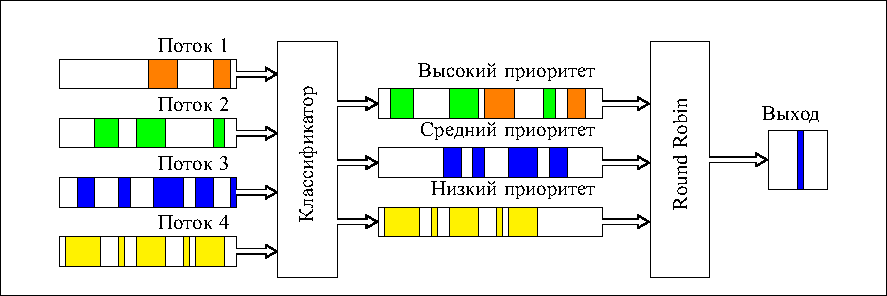
\includegraphics[scale=1.3]{pdfimages/pq.pdf}
        \caption{Схема обслуживания алгоритмом приоритетных очередей}
		\label{pic:pq}
    \end{figure}

    Дисциплина используется, чтобы cнизить время отклика, когда нет нужды замедлять трафик\cite{tcprio}. 

    В Linux алгоритм реализован в виде дисциплины prio, которая создаёт фиксированное
    значение очередей обслуживания (групп или bands), планируемые дисциплиной pfifo\_fast,
	и управляет очередями в соответствии с картой приоритетов.\cite{tcprio}



    Преимущества алгоритма состоят в следующем:
    \begin{itemize}
		\item возможность понижения времени отклика, когда нет необходимости замедлять трафик \cite{tcprio};
        \item наиболее простая в реализации классовая дисциплина обслуживания;
        \item для software-based маршрутизаторов PQ предоставляет относительно небольшую
             вычислительную нагрузку на систему в сравнении с более сложными ДО;
        \item PQ позволяет маршрутизаторам организовывать буферизацию пакетов и обслуживать
             один класс трафика отдельно от других. \cite{suppdiff}
    \end{itemize}

    Однако приоритетные очереди обладают рядом существенных недостатков:
    \begin{itemize}
        \item возникает проблема простоя канала (отсутствие обслуживания в течение продолжительного времени)
			  для низкоприоритетного трафика при избытке высокоприоритетного\cite{packethandling};
        \item избыточный высокоприоритетный трафик может значительно увеличивать
                задержку и джиттер для менее приоритетного трафика;
        \item не решается проблема с TCP и UDP, когда TCP-трафику назначается высокий приоритет и он
                пытается поглотить всю пропускную способность. \cite{suppdiff}
    \end{itemize}

    \subsection{Алгоритм управления очередями на основе классов}

        Алгоритм управления очередями на основе классов (Class Based Queueing, CBQ) -- это
        классовая дисциплина обслуживания, которая реализует иерархическое
        разделение канала между классами и позволяет шейпинг трафика.\cite{tccbq}

        Главная цель CBQ -- это планировка пакетов в очередях, гарантия определённой
        скорости передачи и разделение канала. Если в очереди нет пакетов, её
        пропускная способность становится доступной для других очередей. Сила
        этого метода состоит в том, что он позволяет справляться со значительно
        различными требованиями к пропускной способности канала среди потоков. Это
        реализовано путём назначения определённого процента доступной ширины
        канала каждой очереди. CBQ избегает проблему простоя канала, которой страдает
        алгоритм PQ, так как как минимум один пакет обслуживается от каждой очереди
        в течение цикла обслуживания.\cite{packethandling}

		Алгоритм CBQ представляет канал в виде иерархической структуры \cite{linksharing}
		пример которой представлен на рисунке~\ref{pic:cbq}. Голубым цветом обозначен узел,
		представляющий собой основной канал; он разделяется между двумя классами трафика:
		интерактивным (левый узел) и остальным (правый узел), -- которым назначается процент
		пропускной способности от остального канала. Весь трафик, относящийся к классу,
		будет получать выделенную пропускную способность для этого класса. Эти
		классы трафика могут разделяться на подклассы и так далее. Если класс не использует
		пропускную способность, она будет выделяться классу-соседу. Этот механизм
		называется механизмом разделения канала \cite{linksharing}. 

        \begin{figure}[ht!]
			\center
            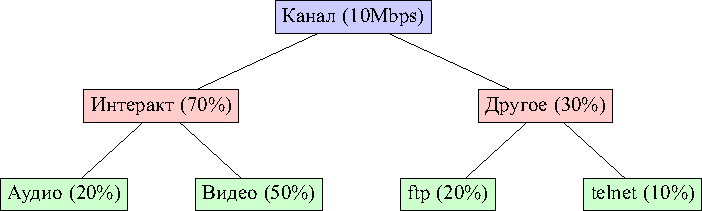
\includegraphics[scale=1.3]{./pdfimages/cbq.pdf}
            \caption{Пример работы механизма разделения канала.}
			\label{pic:cbq}
        \end{figure}

        Алгоритм CBQ состоит в следующем. Сначала пакеты классифицируются в классы
        обслуживания в соответствии с определёнными критериями и сохраняются в
        соответствующей очереди. Очереди обслуживаются циклически. Различное
        количество пропускной способности может быть назначено для каждой очереди
        двумя различными способами: с помощью позволения очереди отправлять более
        чем один пакет на каждый цикл обслуживания или с помощью позволения очереди
        отправлять только один пакет за цикл, но при этом очередь может быть обслужена
        несколько раз за цикл.\cite{packethandling}

		Вычисления в CBQ основываются на вычислении времени в микросекундах между
		запросами, на основе которого рассчитывается средняя загруженность канала;
		в этом и состоит главная проблема неточности CBQ в Linux.\cite{lartc} 

        Преимущества алгоритма состоят в следующем:
        \begin{itemize}
            \item позволяет контролировать количество пропускной способности для каждого
                  класса обслуживания;
            \item каждый класс получает обслуживание, вне зависимости от других классов. Это
                  помогает избегать проблемы PQ, когда при избытке высокоприоритезированного
                  трафика низкоприоритезированный не обслуживался вообще.\cite{packethandling}
        \end{itemize}

        Недостатки же в большей следуют из особенностей реализации алгоритма в системе Linux:
        \begin{itemize}
            \item честное выделение пропускной способности происходит, только если
                  пакеты из всех очередей имеют сравнительно одинаковый размер. Если один класс
                  обслуживания содержит пакет, который длиннее остальных, этот класс обслуживания
                  получит большую пропускную способность, чем сконфигурированное значение \cite{packethandling};

            \item высокая сложность реализации. В ядре Linux реализация СBQ приближённая и
                  в некоторых случаях может давать неверные результаты.\cite{lartc}
        \end{itemize}

    \subsection{Алгоритм иерархического маркерного ведра}

        Алгоритм иерархического маркерного ведра (Hierarchical Token Bucket, HTB) -- дисциплина
        обслуживания с иерархическим разделением канала между классами.

		HTB, подобно CBQ, использует механизм разделения канала. 
		HTB обеспечивает, что количество обслуживания, предоставляемое каждому классу, является,
		минимальным значением из запрошенного количества и назначенного классу. Когда класс
		запрашивает меньше, чем ему выделено, оставшаяся пропускная способность распределяется между
		другими классами, которые требуют обслуживание.\cite{htb}

		Отличительная особенность HTB от CBQ состоит в том, что в HTB принцип работы
		основывается на определении объема трафика\cite{lartc}, что даёт более точные результаты.

		HTB состоит из произвольного числа иерархически организованных фильтров
		маркерного ведра (Token Bucket Filter, TBF)\cite{packethandling},
		однако реализация не использует готовый
		модуль tbf: алгоритм маркерного ядра вcтроен в код реализации
		HTB, что повышает его эффективность. Внутренние классы содержат
		фильтры, которые распределяют пакеты по очередям и метаинформацию
		для разделения канала. Листовые
		классы содержат очереди, которые содержат очереди, которые
		управляются сконфигурированными дисциплинами обслуживания (по
		умолчанию pfifo\_fast). Пример сконфигурированного дерева
		HTB представлен на рисунке~\ref{pic:htb_hier}.
		
        \begin{figure}[ht!]
            \center
            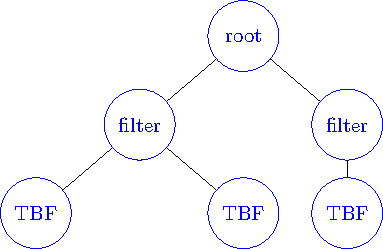
\includegraphics[scale=1.4]{./pdfimages/class_hierh_htb.pdf}
            \caption{Пример иерархии классов при использовании дисциплины HTB}
			\label{pic:htb_hier}
        \end{figure}

        При добавлении пакета в очередь HTB начинает обход дерева от корня
        для определения подходящей очереди: в каждом узле происходит поиск
        инструкций, и затем происходит переход в узел, на который ссылается
        инструкция. Обход заканчивается, когда алгоритм доходит до листа,
        в очередь которого помещается пакет.\cite{tchtb} В реализации алгоритма
		существует прямая очередь, которая используется не только в качестве
		очереди с наивысшем приоритетом, но и как очередь, в которую попадают
		пакеты, не определённые в другую очередь. Это мера не самая удачная,
		но используется для избежания ошибок.

        Преимущества алгоритма HTB приведены ниже.
        \begin{itemize}
            \item Наиболее используемая дисциплина обслуживания в Linux, так как HTB эффективно
				  справляется с обработкой пакетов, а конфигурация HTB легко масштабируется.\cite{lartc}
            \item Иерархическая структура предоставляет гибкую возможность конфигурировать трафик.
            \item Не зависит от характеристик интерфейса и не нуждается в знании о лежащей в
                  основе пропускной способности выходного интерфейса из-за свойств TBF. \cite{tchtb}
            \item Вычислительно проще, чем алгоритм CBQ.\cite{htb}
        \end{itemize}

        Недостатки.
        \begin{itemize}
            \item Медленнее CBQ в N раз, где N -- глубина дерева разделения, что, однако, компенсируется простотой вычислений.\cite{htb}
			\item Нужно что-то ещё весомое.
        \end{itemize}

    \subsection{Алгоритм иерархических честных кривых обслуживания}
% https://www.cs.cmu.edu/~hzhang/papers/SIGCOM97.pdf
% http://linux-tc-notes.sourceforge.net/tc/doc/sch_hfsc.txt
% https://serverfault.com/questions/105014/does-anyone-really-understand-how-hfsc-scheduling-in-linux-bsd-works

        HFSC (Hierarchical Fair-Service Curve) -- иерархический алгоритм планирования пакетов,
        основанный на математической модели честных кривых обслуживания (Fair Service Curve),
        где под термином "кривая обслуживания" подразумевается зависящая от времени
        неубывающая функция, которая служит нижней границей количества обслуживания,
        предоставляемого системой.\cite{hfsc}

        HFSC ставит перед собой цели:
        \begin{itemize}
            \item гарантировать точное выделение пропускной способности и задержки для всех листовых классов (критерий реального времени);
            \item честно выделять избыточную пропускную способность так, как указано классовой иерархией (критерий разделения канала);
            \item минимизировать несоответствие кривой обслуживания идеальной модели и действительного количество обслуживания.\cite{tchfsc}
        \end{itemize}

        Алгоритм планировки основан на двух критериях: критерий реального времени
        (real-time) и критерий разделения канала (link-sharing). Критерии реального времени
        используются для выбора пакета в условиях, когда есть потенциальная опасность,
        что гарантия обслуживания для листового класса нарушается. В ином случае
        используется критерий разделения канала.\cite{tchfsc}

		\begin{figure}[ht!]
		 	\center
            \begin{subfigure}[b]{0.3\textwidth}
                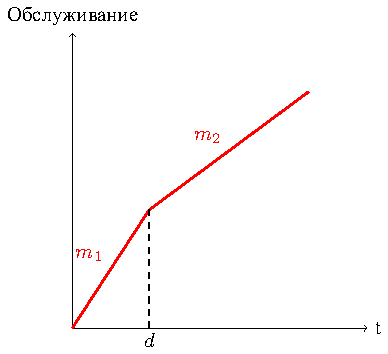
\includegraphics[width=\textwidth]{pdfimages/hfsc_concave.pdf}
                \caption{Вогнутая кривая.}
                \label{pic:hfsc_concave}
            \end{subfigure}
            \hspace{0.2\textwidth}
            \begin{subfigure}[b]{0.3\textwidth}
                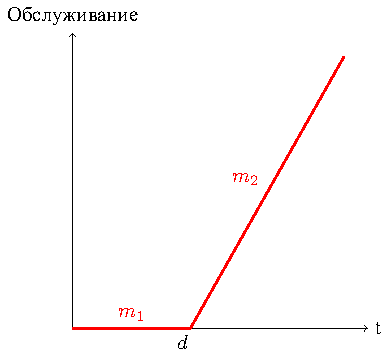
\includegraphics[width=\textwidth]{pdfimages/hfsc_convex.pdf}
                \caption{Выпуклая кривая.}
                \label{pic:hfsc_convex}
            \end{subfigure}
			\caption{Примеры кривых обслуживания. $m_1$ -- скорость в стационарном состоянии,
			$m_2$ -- скорость в режиме burst, $d$ -- время, за которое происходит передача
			в режиме burst.\cite{hfscguide}}
			\label{pic:hfscline}
        \end{figure}

		На рисунке~\ref{pic:hfscline} изображены примеры кривых обслуживания, используемых
		в дисциплине HFSC; параметры $m_1$, $m_2$ и $d$, отображённые на графиках, задаются
		при конфигурации дисциплины.\cite{hfscguide}

        HFSC использует три типа временных параметров: время крайнего срока (deadline
        time), "подходящее" время (eligible time) и виртуальное время (virtual time). Время крайнего
        срока назначается таким образом, чтобы, если крайние сроки всех пакетов сессии
        выполнены, его кривая была гарантирована. "Подходящее" время используется для
        выбора критерия планировки для следующего пакета. Виртуальное время показывает
        нормализованное количество обслуживания, которое получил класс. Виртуальное
        время присуще всем вершинам дерева классов, так как является важным параметром
        при критерии разделение канала, при котором должно минимизироваться
        несоответствие между виртуальным временем класса и временами его соседей
        (так как в идеальной модели виртуальное время соседей одинаково); при выборе
        критерия разделения канала алгоритм рекурсивно, начиная с корня, обходит всё
        дерево, переходя в вершины с наименьшим виртуальным временем. Время крайнего
        срока и <<подходящее>> время используются дополнительно в листовых классах,
        так как в этих вершинах непосредственно содержатся очереди.\cite{hfsc}

		Основное преимущество алгоритма состоит в том, что он основан
		на формальной модели с доказанными нижними границами. Он даёт гарантированные
		результаты и вычисляет более точно, чем дисциплины CBQ и HTB, которые
		служат схожим целям.

		Главные же недостатки HFSC заключены в его достоинстве. Алгоритм основан
		на формальной модели и имеет множество параметров, требующих дополнительных
		расчётов и времени на подготовку к конфигурации. Также он довольно сложен
		в реализации и поддержке. 

    \subsection{Взвешенный алгоритм честного обслуживания очередей}

    WFQ (Weighted Fait Queueing) -- динамический метод планировки пакетов, который
    предоставляет честное разделение пропускной способности всем потокам трафика.
    WFQ применяет вес, чтобы идентифицировать и классифицировать трафик
    в поток и определить, как много выделить пропускной способности каждому
    потоку относительно других потоков. WFQ на месте планирует интерактивный трафик в начало очереди,
    уменьшая там самым время ответа, и честно делит оставшуюся пропускную
    способность между остальными потоками. \cite{ciscoguide}
    % https://www.cisco.com/c/en/us/td/docs/ios/12_2/qos/configuration/guide/fqos_c/qcfconmg.html


	WFQ представляет собой аппроксимацию обобщённой схемы разделения 
	процессорного времени (General Processor Sharing, GPS). GPS
	-- это схема, обеспечивающая честное обслуживание по типу
	взвешенной максиминной схемы равномерного распределения ресурсов
	(схема, при которой каждому пользователю назначается определённый вес
	и выделяется равномерная доля ресурсов, пропорциональная этому весу).
	В соответствии со схемой GPS каждый поток трафика помещается в
	собственную логическую очередь, после чего бесконечно малый объём
	данных из каждой непустой очереди обслуживается по круговому принципу.
	Необходимость обработки бесконечно малого объёма данных на каждом
	круге обусловлена требованием обслуживания всех непустых очередей
	на любом конечном временном интервале. Из-за чего схема GPS является
	справедливой в любой момент времени. Однако технически
	невозможно реализовать данную схему на практике; WFQ же
	предлагает брать за рабочую единицу пакет.\cite{Vagesna}

	Алгоритм WFQ использует концепцию виртуального времени, чтобы
	отслеживать расчёты схемы GPS. В рамках этой концепции
	используется понятие события $j$, которое обозначает
	прибытие или отправление пакета во время $t_j$.
	Виртуальное время идёт не с той же скоростью, с какой
	идёт реальное; его скорость зависит от активных потоков в рассматриваемый реальный промежуток времени.
	Разница представлена на рисунке~\ref{pic:wfqtime}.

    \begin{figure}[ht!]
		\center
        \includegraphics[scale=1.3]{./pdfimages/wfq_time.pdf}
        \caption{Сравнение движений реального и виртуальных времён.}
		\label{pic:wfqtime}
    \end{figure}

	По Формуле (\ref{eq:virtualtime}) рассчитывается движение виртуального
	времени в GPS. Скорость виртуального времени зависит от количества активных сессий.
	%количество обслуживания, которая
	%очередь должна получить в соответствии с моделью GPS.
 
    \begin{gather}
		\label{eq:virtualtime}
			V_{t_{j - 1} + \tau} = V_{t_{j - 1}} + \dfrac {\tau} {\sum \limits_{i \in B_{j}} w^{i}}, \tau \leq t_j - t_{j - 1}\\
			V(0) = 0
        \intertext{где}
            {\renewcommand\arraystretch{1.25}
            \begin{tabular}{>{$}l<{$}@{\ ---\ }ll}
            w^{i} & \multicolumn{2}{p{12cm}}{вес потока i.}\\
            B_j   & \multicolumn{2}{p{12cm}}{обозначает, является ли поток на данный момент активным.}
            \end{tabular}} \nonumber
    \end{gather}

	Виртуальное время завершения обслуживания обозначает виртуальное время, когда должно завершиться
	обслуживания в соответствии со схемой GPS. Пакет с наименьшим виртуальным временем первым	
	покинет систему обслуживания. Для вычисления виртуального времени завершения обслуживания
	по Формуле (\ref{eq:finishtime}) необходимо вычислить виртуальное время начала
	обслуживания по Формуле (\ref{eq:starttime}).

    \begin{gather}
		\label{eq:starttime}
    		S_i^k = \max\{F_i^{k - 1}, V_{a_i^k} \},
        \intertext{где}
            {\renewcommand\arraystretch{1.25}
            \begin{tabular}{>{$}l<{$}@{\ ---\ }ll}
            S_i^k & \multicolumn{2}{p{12cm}}{виртуальное время начала обработки пакета под номером $k$ из потока $i$.}\\
            F_i^k & \multicolumn{2}{p{12cm}}{виртуальное время конца обработки пакета под номером $k$ из потока $i$.}\\
            %V_{a}    & \multicolumn{2}{p{12cm}}{нормализованное честное количество времени обслуживания,
			%								    которая каждая очередь должна получить в соответствии с моделью GPS
			%									(Формула~\ref{eq:virtualtime}).}\\
            a_i^k & \multicolumn{2}{p{12cm}}{время прибытия пакета под номером $k$ из потока $i$.}
            \end{tabular}} \nonumber
    \end{gather}

    \begin{gather}
		\label{eq:finishtime}
			F_i^k = S_i^k + \dfrac {L_i^k} {w_i},\\
			F_i^0 = 0,\nonumber
        \intertext{где}
            {\renewcommand\arraystretch{1.25}
            \begin{tabular}{>{$}l<{$}@{\ ---\ }ll}
            L_i^k & \multicolumn{2}{p{12cm}}{длина пакета под номером $k$ из потока $i$.}\\
            w_i      & \multicolumn{2}{p{12cm}}{вес потока $i$.}\\
            \end{tabular}} \nonumber
    \end{gather}

	В Таблице~\ref{tab:wfqexpl} приведён пример вычисления виртуального времени завершения
	обслуживания. По столбцу $F$ видно, что систему раньше покинут пакеты с большим
	весом.
	\begin{table}[ht!]
		\center
		\caption{Пример вычисления времени завершения обслуживания.}
		\label{tab:wfqexpl}
		\begin{tabular}{|c|c|c|c|c|c|c|c|}
		\hline
                     & \multicolumn{3}{c|}{Поток 1}     & \multicolumn{3}{c|}{Поток 2} \\ \hline
            Вес      & \multicolumn{3}{c|}{$w_1 = \dfrac{1} {3}$} & \multicolumn{3}{c|}{$w_2 = \dfrac {2} {3}$} \\ \hline
        Номер пакета & $a_1$ & $L_1$ & $F_1$& $a_2$ & $L_2$ & $F_2$ \\ \hline
                1    &   1   &   1   &  4   &   0   &  3    & 4 \\ \hline 
                2    &   2   &   1   &  5   &   3   &  2    & 8 \\ \hline 
                3    &   4   &   2   &  9   &   5   &  2    & 14  \\ \hline 
                4    &   7   &   2   &  13  &   -   &  -    & -  \\ \hline 
		\end{tabular}

	\end{table}

	Для отправки каждый цикл обслуживания выбирается пакет с наименьшим виртуальным временем конца обработки.
	Итоговая пропускная способность $r_i$ рассчитывается на основе заданных весов по Формуле~\ref{eq:rate}\cite{pgps}
    \begin{gather}
		\label{eq:rate}
			r_i = \dfrac{w_i} {\sum \limits_{i = 0}^{N} w_i} \cdot R
        \intertext{где}
            {\renewcommand\arraystretch{1.25}
            \begin{tabular}{>{$}l<{$}@{\ ---\ }ll}
            w_i & \multicolumn{2}{p{12cm}}{вес, назначенный потоку $i$.}\\
            N   & \multicolumn{2}{p{12cm}}{количество потоков.}\\
            R   & \multicolumn{2}{p{12cm}}{полная пропускная способность канала.}\\
            \end{tabular}} \nonumber
    \end{gather}

	Рассмотрим алгоритм WFQ на основе потока (Flow-based WFQ, FWFQ). Название алгоритма отсылает к методу
	классификации пакетов, при котором очередь выделяется для пакетов одного потока.\cite{Vagesna}
	Схема планировщика представлена на рисунке~\ref{pic:fwfqscheme}.

    \begin{figure}[ht!]
		\center
        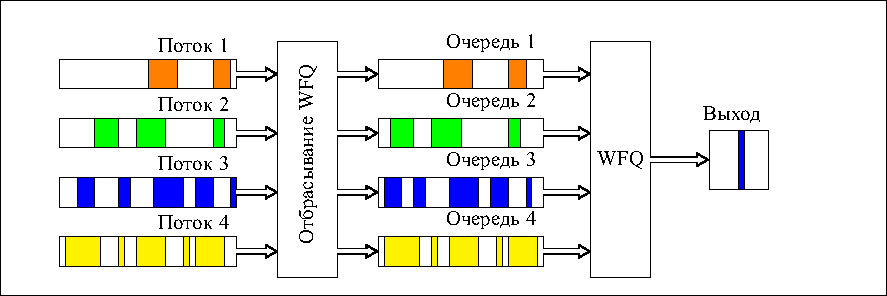
\includegraphics[scale=1.3]{./pdfimages/fwfq.pdf}
        \caption{Схема WFQ системы на основе потоков.}
		\label{pic:fwfqscheme}
    \end{figure}

	В реализации FWFQ от Cisco используется алгоритм WFQ на основе порядкового номера
	пакета. Алгоритм поддерживает два счётчика: счётчик цикла, который 
	определяет количество пройденных циклов побайтового планировщика (и равняется
	порядковому номеру последнего обслуженного пакета), и значение
	наибольшего порядкового номера пакета, поставленного в очередь потока.
	На основе этих значений высчитывается порядковый номер пакета, пакет
	с минимальным значением покидает систему. Вычисление порядкового номера пакета
	вычисляется в зависимости от того, активный ли поток на момент прибытия нового пакета.
	Если поток был неактивным, то $\textit{порядковый номер пакета} = \textit{размер пакета в байтах} \cdot \textit{вес}
	+ \textit{значение счётчика цикла на момент поступления пакета}$; если поток активный,
	то $\textit{порядковый номер пакета} = \textit{размер пакета в байтах} \cdot \textit{вес}
	+ \textit{значение наибольшего порядкового номера пакета в потоке}$.
	Веc пакета строко зависит от его приоритета (определяется по соответствующему полю заголовка IP)
	и не может быть изменён.\cite{Vagesna} Условная схема работы алгоритма представлена на
	рисунке~\ref{pic:wfqseq}.

    \begin{figure}[ht!]
		\center
        \includegraphics{./pdfimages/wfq_seq.pdf}
        \caption{Условная схема работы алгоритма WFQ на вычисления порядкового номера.}
		\label{pic:wfqseq}
    \end{figure}

    Планировщик не нарушает порядка обработки пакетов, принадлежащих одному
    потока, даже в том случае, если они имеют различный приоритет.
    В целях планировки в WFQ длина очереди измеряется не в пакетах, а во времени,
    которое заняла бы передача всех пакетов в очереди.\cite{Vagesna}

	%WFQ адаптирует количество
    %потоков и выделяет одинаковое количество полосы пропускания каждому потоку.
    %Поток с маленькими пакетами, которые обычно являются интерактивными потоками,
    %получают лучшее обслуживание, потому что они не нуждаются в большой полосе пропускания;
    %также они получаются низкую задрежку, потому что у меньших пакетов меньшее
    %время отправки (finish time). Время отправки -- это сумма текущего времени и
    %время, которое заняла бы отправка пакета. Текущее время ноль, если в очереди
    %нет пакетов. WFQ поместит пакет в аппаратную очередь, основываясь на времени отправки в
    %порядке возрастания.
	

    WFQ использует два метода отбрасывания пакетов: ранее (Early Dropping) и агрессивное
    (Aggressive Dropping) отбрасывания. Ранее отбрасывание срабатывает тогда, когда
    достигается congestive discard threshold (CDT); CDT -- это количество пакетов, которые могут
    находиться в системе WFQ перед тем, как начнётся отбрасывание новых пакетов
    из самой длиной очереди; используется, чтобы начать отбрасывание пакетов
    из наиболее агрессивного потока, даже перед тем, как он достигнет предел
    hold queue out (HQO). HQO -- это максимальное количество пакетов, которое может быть
    во всех выходящих очередях в интерфейсе в любое время; при достижении HQO
    срабатывает агрессивный режим отбрасывания. Алгоритм представлен на рисунке~\ref{pic:wfqdropalgo}.
    \cite{wfqdrop}

    \begin{figure}[ht!]
			\center
        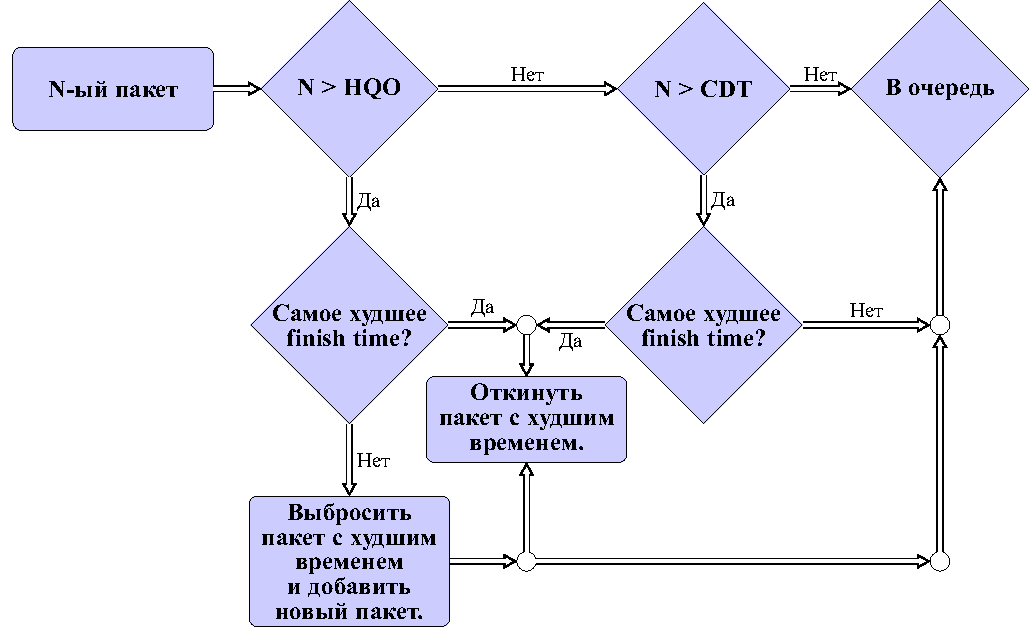
\includegraphics{./pdfimages/fwfq_drop.pdf}
        \caption{Схема отбрасывания пакетов WFQ.}
		\label{pic:wfqdropalgo}
    \end{figure}

    Преимущества WFQ.
    \begin{itemize}
        \item Простая конфигурация.
        \item Отбрасывание пакетов из более агрессивных потоков, что предотвращает перегрузки.
		\item Из-за честного обслуживания отсутствует проблема голодания потоков.
    \end{itemize}

    WFQ страдает от нескольких недостатков.
    \begin{itemize}
        \item Трафик не может регулироваться на основе достигнется  определённых классов обслуживания.
        \item Не поддерживает задание определённой пропускной способности для типа трафика.
		\item В Cisco системах WFQ поддерживается только на медленных каналах.\cite{wfqdis}
    \end{itemize}

    Эти ограничения были исправлены CBWFQ.

    \subsection{Взвешенный алгоритм честного обслуживания очередей на основе классов}

    % https://www.cisco.com/en/US/docs/ios/12_0t/12_0t5/feature/guide/cbwfq.html
%   Надо описать, что было создано в Cisco и т.п. и как это работает в циско.
%   Таблица сравнений с flow-based WFQ
%   Предоставляет одну очередь для класса, всего 64 класса.
%   Позволяет указывать пропускную способность для класса
%   Предоставляет гарантию пропускной способности для пользовательких классов.
%   Предоставляет поддержку flow-based WFQ для не определёнными пользователями
%   трафиков класса.
%   Требует конфигурацию.
%   [cм ссылку в комментах]
    % https://www.cisco.com/c/en/us/td/docs/ios/12_2/qos/configuration/guide/fqos_c/qcfconmg.html

    CBWFQ (Class-based weighted fair queueing) -- основанный на классах взвешенный алгоритм равномерного обслуживания 
    очередейc\cite{Vagesna}; является расширением функциональности дисциплины обслуживания WFQ,
    основанной на потоках, для предоставления определяемых пользователями классов трафика. 

    Сlass-Based WFQ -- это мехaнизм, использующийся для гарантировании пропускной способности
    для класса. Для CBWFQ класс трафика определяется на основе заданных критериев
    соответствия: список контроля доступа (ACL), протокол, входящий интерфейс и т.п. Пакеты,
    удовлетворяющие критериям класса, составляют трафика для этого класса. Дисциплина
    позволяет задавать до 64-х пользовательских классов.
		
	Схема дисциплины обслуживания представлена на рисунке~\ref{pic:cbwfqscheme}. 

 	\begin{figure}[ht!]
		\center
    	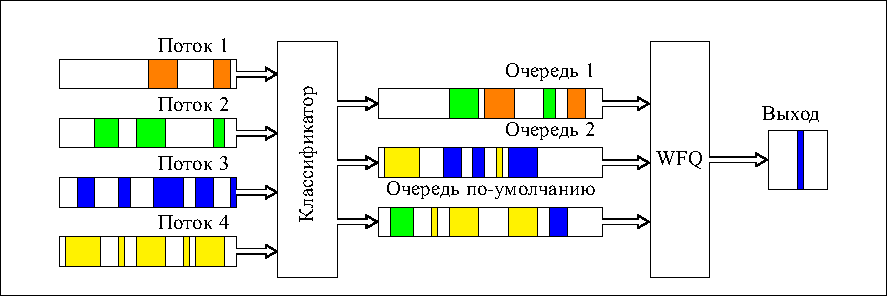
\includegraphics[scale=1.3]{pdfimages/cbwfq.pdf}
		\caption{Схема дисциплины обслуживания CBWFQ.}
		\label{pic:cbwfqscheme}
	\end{figure}   

    После определения класса, ему назначаются характеристики, которые определяют
    политику очереди: пропускная способность, выделенная классу, максимальная
    длина очереди и так далее. Алгоритм CBWFQ позволяет явано указать требуемую минимальную
    полосу пропускания для каждого класса трафика. Полоса пропускания используется
    в качестве веса класса. Вес можно задать в абсолютной (опция \texttt{bandwidth}),
    в процентной (опция \texttt{bandwidth percent}) и в доле от оставшиейся
    полосы пропускания (опция \texttt{bandwidth remaining precent}) величинах.
    Кроме пользовательских классов CBWFQ предоставляет стандартный класс (default class),
    в который попадает весь трафик, который не был классифицирован. В стандартном классе
    управление очередью может осуществляться с помощью алгоритмов FIFO и FQ (Fair Queueing). \cite{ciscoguide} 

    В случае переполнения очередей начинает работать алгоритм отбрасывания пакетов.
    В качестве политики отбрасывания пакетов по умолчанию используется отбрасывание конца
    очереди (Tail Drop), однако допускается сконфигуривать работу
    алгоритм взвешенного произвольного раннего обнаружения (Weighted Random Early Detection, WRED)
    для каждого класса.\cite{ciscoguide}

	Преимущества:
	\begin{itemize}
		\item позволяет явно задать полосу пропускания для класса;
		\item позволяет создавать классы трафика и настраивать их в соответствии с требованиями;
		\item простая конфигурация вследствие небольшого числа параметров.\cite{Vagesna}\cite{ciscoguide}
	\end{itemize}

	Недостатки:
	\begin{itemize}
		\item нет поддержки работы с интерактивным трафиком (что исправляется в дисциплине обслуживания Low Latency Queueing (LLQ),
		которая является развитием CBWFQ);
		\item в Cisco реализации наблюдается ограничение на количество пользовательских классов (до 64-х классов);\cite{Vagesna}
		\item отсутствие открытой реализации, что усложняет реализацию алгоритма в других системах и требует его полного воссоздания
		на основе имеющихся источников.
	\end{itemize}

	\subsection{Выводы}

	\begin{table}[ht!]
		\center
    	\caption{Сравнительная таблица дисциплин обслуживания.}
		\label{tab:compqdisc}
        \begin{tabular}{|>{\rowmac}c|>{\rowmac}c|>{\rowmac}c|>{\rowmac}c|>{\rowmac}c|>{\rowmac}c|>{\rowmac}c<{\clearrow}|}
            \hline
            \setrow{\bfseries}     Свойство        & PQ   & CBQ   & HTB   & HFSC  & FWFQ  & CBWFQ \\ \hline
            {\bf \mc{Метод\\ планирования        }}& RR   & WRR   & RR    & RT/LS & WFQ   & WFQ   \\ \hline
            {\bf Отбрасывание                     }& TD   & TD    & TD    & TD    & ED/AD & TD/WRED \\ \hline
            {\bf \mc{Честность\\(справедливость) }}& -    & -     & -     & -     &  +    &  +    \\ \hline
            {\bf \mc{Разделение\\ канала         }}& -    &  +    &  +    &  +    &  -    &  -    \\ \hline
			{\bf \mc{Решение проблемы\\ голодания}}& -    &  +    & +     & +     & +     & +    \\ \hline
            {\bf \mc{Сложность \\ реализации     }}& Низк & Выс   &Сред   & Выс   & Сред  & Сред \\ \hline
            {\bf \mc{Сложность \\ конфигурации   }}& Низк & Выс   &Сред   & Выс   & Низк  & Низк \\ \hline
            {\bf \mc{Конфигурация\\ классов      }}& -    & +     & +     & +     & -     & + \\ \hline
            {\bf \mc{Реализация\\ в Linux        }}& +    & +     & +     & +     & -     & -  \\ \hline
        \end{tabular}

		%Обозначения: RR -- Round Robin (алгоритм циклического
    	%обслуживания), WRR -- Weighted Round Robin (алгоритм взвешенного циклического обслуживания), RT/LS --
    	%Real-Time/Link-Sharing (алгоритм, который обслуживает очередь в зависимости от критерия реального времени
    	%и критерия разделения канала), TD -- Tail Drop (алгоритм обрасывания "хвостов"), ED/AD --
    	%Early-Detection/Aggressive-Detection (алгоритм раннего и агрессивного обнаружения),
    	%WRED -- Weighted Random Early Detection (алгоритм взвешенного раннего обнаружения)}
	\end{table}
	Каждая из рассмотренных ДО обладает своими достоинствами и недостатками. В Таблице~\ref{tab:compqdisc}
	приведено сравнение основных элементов проанализированных дисциплин обслуживания.

	Особое внимание следует уделить механизмам честного обслуживания и
	разделения канала. Оба метода служат решением проблемы голодания,
	однако используют разные по сложности подходы. Механизм разделения канала
	использует сложные вычисления и требует не только тщательной реализации
	и поддержки (что явно видно при исследовании исходного кода
	приведённых выше дисциплин CBQ, HTB и HFSC), но и кропотливой конфигурации. 
	В то время, когда честное обслуживание не требует реализации сложных механизмов.
	У него есть свои недостатки: оно не позволяет построения сложных иерархических
	связей и разделения пропускной способности между классами одного уровня. 
	Однако это требуется не во всех ситуация; для простой конфигурации
	в нетривиальных, но не требующих тщательного контроля, случаях
	лучше всего использовать несложные в конфигурации механизмы, дающие
	схоЖий результат. Поэтому реализация CBWFQ в ядре Linux целесообразна.


	% Chapter 2: исследование CBWFQ в системах моделирования
	\newpage
	\section{ТЕСТИРОВАНИЕ РАЗРАБОТАННОГО МОДУЛЯ ДИСЦИПЛИНЫ ОБСЛУЖИВАНИЯ CLASS-BASED WFQ}

	\subsection{Описание тестовой среды}

		Для тестирования модуля ядра была создана система виртуальных машин на основе
		системы эмуляции программного обеспечения QEMU. Схема тестовой среды представлена
		на Рисунке~\ref{pic:testscheme}. Источником служит узел, от которого исходит трафик;
		таблицы маршрутизации настроены таким образом, чтобы весь трафик, который
		должен попасть на узел-цель шёл через промежуточный узел, на котором
		настроена тестируемая дисциплина обслуживания CBWFQ.

        \begin{figure}[ht!]
        	\center
        	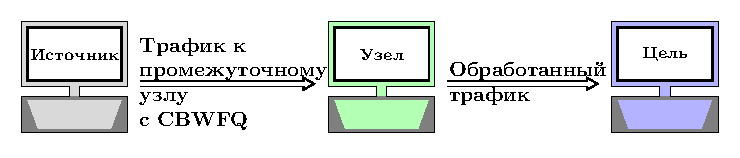
\includegraphics[scale=1.2]{pdfimages/test_scheme.pdf}
        	\caption{Схема тестовой среды.}
			\label{pic:testscheme}
        \end{figure}

		В Листинге~\ref{lst:tccmd} приведена система настройки дисциплины на промежуточном узле.

		Переменная окружения \lstinline{TESTPORT} содержит в себе номер порта,
		с которого будет отправлен трафик на сервер. При добавлении дисциплины
		на интерфейс необходимо указать пропускную способность канала; размер
		очереди по умолчанию назначается опционально. При конфигурации класса
		во второй строке происходит назначения полосы пропускания для класса
		в процентах (возможно также назначение в bps).
        Так как CBWFQ всегда имеет класс по умолчанию, то
		при добавлении нового класса классу по умолчанию будет доставаться
		оставшаяся пропускная способность.
        В третьей строке происходит
		назначение фильтра, который будет направлять трафик с исходным портом \lstinline{TESTPORT}
		в очередь класса 1:2. На один класс можно назначит множество фильтров
		(Linux предоставляет гибкие возможности по настройке фильтрации); это не
		контролируется непосредственно дисциплиной и находится в компетенции
		пользователя. 

        \begin{figure}[ht!]
    		\center
    		\begin{lstlisting}[frame=lines,
    						  caption={Список команд для конфигурации дисциплины обслуживания CBWFQ.},
    						  label={lst:tccmd},
    						  style=tcstyle]

tc qdisc add dev $IFACE root handle 1: cbwfq bandwidth 100Mbps\
        default rate 5Mbps


tc class add dev $IFACE parent 1: classid 1:2 cbwfq rate 35Mbps
tc class add dev $IFACE parent 1: classid 1:3 cbwfq rate 70Mbps

tc filter add dev ens4 parent 1:1 protocol ip u32 match \
        ip dport $TESTPORT1 0xffff flowid 1:2

tc filter add dev ens4 parent 1:0 protocol ip u32 match \
        ip dport $TESTPORT2 0xffff flowid 1:3
    		\end{lstlisting}
        \end{figure}

		\subsection{Анализ точности выделения канала при конкурирующем трафике}
			
			Первый эксперимент заключается в исследовании разделения канала между
			двумя потоками трафика, приходящими со скоростью, больше скорости канала на
			промежуточном узле.

    		С использованием описанной конфигурации и указанных в Листингах~\ref{lst:iperfsrc} и~\ref{lst:iperfdst}
			команд произвелось десять испытаний в рамках эксперимента (схема
			эксперимента представлена на Рисунке~\ref{pic:exp1}).

    		В течение экспериментов собирались отчёты от утилиты iperf со стороны сервера в
    		течение 90-та секунд. Отчёты представляют собой таблицу с полями:
			временной интервал (в секундах), количество переданных данных и пропускная способность.
			На каждый временной интервал таблица содержит описанную информацию для двух потоков.

        \begin{figure}[ht!]
    		\center
    		\begin{lstlisting}[frame=lines,
    						  caption={Команда iperf на узле-источнике (клиентская сторона).},
    						  label={lst:iperfsrc}]
iperf3 -c $SERVERIP -p $TESRPORT1 -b 500M -u -t 90
iperf3 -c $SERVERIP -p $TESRPORT2 -b 500M -u -t 90
    		\end{lstlisting}
        \end{figure}	
        \begin{figure}[ht!]
    		\center
    		\begin{lstlisting}[frame=lines,
    						  caption={Команда iperf на узле-цели (серверная сторона).},
    						  label={lst:iperfdst}]
iperf3 -s -p $TESTPOR1 --logfile class2"$EXPNUM".log
iperf3 -s -p $TESTPOR2 --logfile class3"$EXPNUM".log
    		\end{lstlisting}
        \end{figure}


			Результаты эксперимента можно наблюдать на Рисунке~\ref{pic:plot}. Доля пропускной
			способности для первого и второго класса соответствует минимальной сконфигурированной доле, выделенной
			этим классам (или их весу $\dfrac{\text{70Mbps}}{\text{100Mbps}} = 0.7$ и
            $\dfrac{\text{35Mbps}}{\text{100Mbps}} = 0.35$ соответственно). 

            \begin{figure}[ht!]
            	\center
            	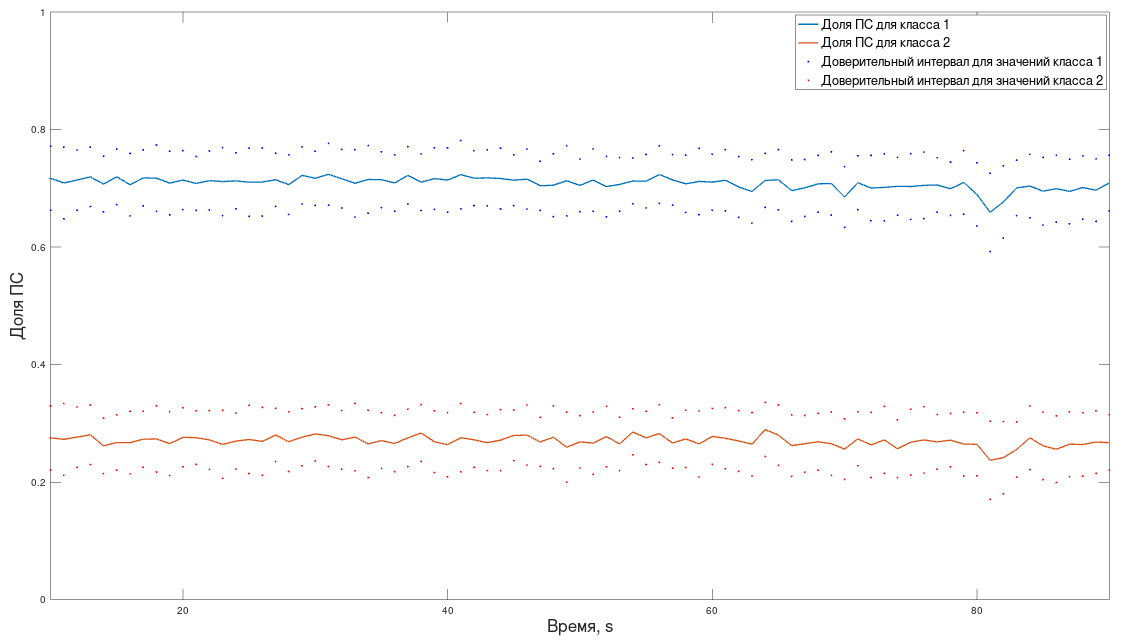
\includegraphics[width=1\linewidth]{./plotc.png} %{pdfimages/plots/plot_comet.pdf}
            	\caption{График распределения доли пропускной способности (ПС) по типам трафика в течение времени.
						 Среднее значение процента ПС для класса 1: $71 \pm 3 \% (P = 0.95)$.
                         Среднее значение процента ПС для класса 2: $37 \pm 2 \% (P = 0.95)$.
                        }
    			\label{pic:plot}
            \end{figure}

		\subsection{Анализ точности выделения канала при независимом трафике}

			Второй эксперимент заключается в исследовании разделения канала между
			двумя потоками трафика, приходящими со скоростью, суммарно меньше
			скорости канала и соответствующие конфигурационным параметрам.

    		С использованием описанной конфигурации и указанных в Листингах~\ref{lst:iperfsrc2} и~\ref{lst:iperfdst2}
			команд произвелось десять испытаний в рамках эксперимента (схема
			эксперимента представлена на Рисунке~\ref{pic:exp2}).

    		В течение экспериментов собирались отчёты от утилиты iperf со стороны сервера в
    		течение 90-та секунд. Отчёты представляют собой таблицу с полями:
			временной интервал (в секундах), количество переданных данных и пропускная способность.
			На каждый временной интервал таблица содержит описанную информацию для двух потоков.


        \begin{figure}[ht!]
    		\center
    		\begin{lstlisting}[frame=lines,
    						  caption={Команда iperf на узле-источнике (клиентская сторона).},
    						  label={lst:iperfsrc2}]
iperf3 -c $SERVERIP -p $TESRPORT1 -b 100M -u -t 90
iperf3 -c $SERVERIP -p $TESRPORT2 -b 5M -u -t 90
    		\end{lstlisting}
        \end{figure}	
%$
        \begin{figure}[ht!]
    		\center
    		\begin{lstlisting}[frame=lines,
    						  caption={Команда iperf на узле-цели (серверная сторона).},
    						  label={lst:iperfdst2}]
iperf3 -s -p $TESTPOR1 --logfile class2"$EXPNUM".log
iperf3 -s -p $TESTPOR2 --logfile class3"$EXPNUM".log
    		\end{lstlisting}
%$
        \end{figure}

			Результаты эксперимента можно наблюдать на Рисунке~\ref{pic:plot2}. В данном
			случае второй класс получает всю требуемую ему пропускную способность; в этом
			факте и состоит отсутствие конкуренции: второй поток не пытается занять больше,
			чем ему назначенно. Поток первого класса занимает оставшуюся свободную часть канала.
			
            \begin{figure}[ht!]
            	\center
            	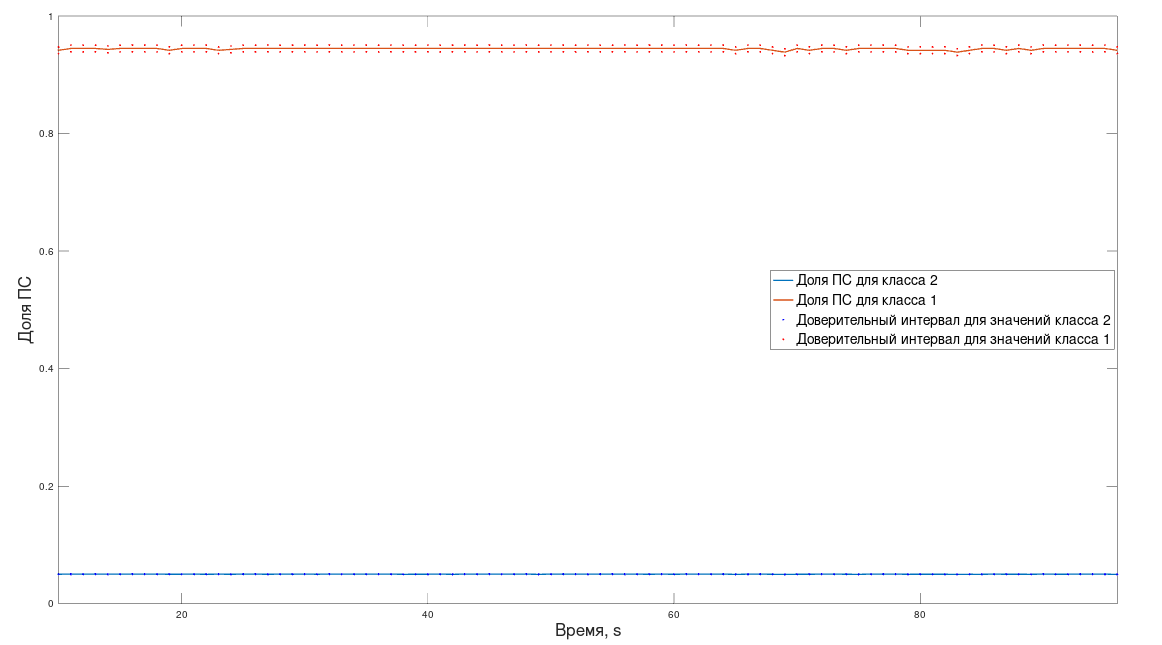
\includegraphics[width=\linewidth]{./plotnc.png} %{pdfimages/plots/plot_no_compet.pdf}
            	\caption{График распределения доли пропускной способности (ПС) по типам трафика в течение времени.
						 Среднее значение процента  ПС для класса 1: $94 \pm 0.5 \%(P = 0.95)$.
                         Среднее значение процента  ПС для класса 2: $5 \pm 0.07 \%(P = 0.95)$}
    			\label{pic:plot2}
            \end{figure}


	% Chapter 2: Описание реализации и тестирования
	\newpage
	\section{Реализация Class-Based WFQ в ядре Linux}

	\subsection{Управление трафиком}

	%Расскать про traffic control (tc) и как он связан с конфигурацией qdisc + Netlink.

	В Linux управление трафиком осуществляется с помощью подсистемы Traffic Control,
	которая предоставляет пользовательский интерфейс с помощью программы \texttt{tc}.
	\texttt{tc} -- это пользовательская программа, которая позволяет настраивать
	дисцплины обслуживания в Linux. Она использует Netlink в качестве
	коммуникационного канала для взаимодействия между пользовательским
	пространством и пространством ядра. Он добавляет новые дисциплины
	обслуживания, классы трафика, фильтры и предоставляет команды для
	управление всеми обозначенными объектами.
	% TCP-IP architecture

	\texttt{tc} предоставляет интерфейс для дисцплины обслуживания,
	представленный структурой \lstinline{struct qdisc_util}, которая
	описывает функции для отправления входящих параметров и печати
	сообщений от ядра. Сообщение, помимо общей информации для подсистемы,
	содержит специфичную для дисциплины структуру с опциями, описываемую
	в заголовке ядра (pkt\_sched.h). 

	Таком образом, для использования дисциплины обслуживания необходимо
	реализовать интерфейс в системе \texttt{tc}. 

	\subsection{Алгоритм выделения канала} 

	???

	\subsection{Описание устройства подсистемы планировки в ядре Linux}
	% Информация из комментариев к ним.
	% Файлы: linux/net/sched/sch_api.c, linux/include/net/{sch_generic.h,pkt_sched.h}. 

	%[Схема пути пакета]

	%В ядре сетевое устройство описывается структурой \lstinline{struct net_device},
	%которая содержит указатель на ассоциированную с устройством дисциплину обслуживания,
	%описываемая структурой \lstinline{struct Qdisc}.

	%Опишем важные для понимания подсистемы поля \texttt{Qdisc}.
	%\begin{itemize}
	%	\item enqueue
	%\end{itemize} 

	В общем случае, дисциплина обслуживания -- это чёрный ящик, который может
	ставить пакеты в очереди и вынимать их из очереди, когда устройство
	готово к отправке, в порядка и во время, определёнными спрятанным в ящике
	алгоритмом. В ядре Linux дисциплины обслуживания представляются в качестве
	модулей ядра, которые реализуют предоставляемый ядром интерфейс.

	Linux поддерживает классовые и бесклассовые дисцплины обслуживания. Примером
	бесклассовой дисциплины служит pfifo\_fast, классовой -- HTB.

	% lartc

	Классы представляют собой одельные сущности в иерархии основной дисциплины.
	Если структура представляет собой дерево, то в классах-узлах могут содержаться
	фильтры, которые определят пакет в нужный класс-потомок. В классах-листьях
	непосредстенно располагаются очереди, которые управляются внутренней дисциплной
	обслуживания (обычно это FIFO). 

	Каждый интерфейс имеет корневую дисцплину (по умолчанию pfast\_fifo), которой
	назначается идентификатор (handle), который используется для обращения к дисциплине.
	Этот идентификатор состоит из двух частей: мажорной (MAJ) и минорной (MIN); мажорная
	часть определяет родителя, минорная -- непосредственно класс.

	\begin{figure}[ht!]
		\centering
		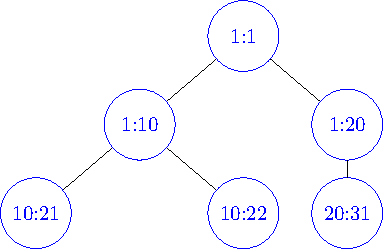
\includegraphics{./pdfimages/class_hierh.pdf}
		\caption{Схема классовой иерархии с использованием идентификаторов MAJ:MIN}
	\end{figure}

	[Возможно, сделать небольшой вывод по описанному и связать его со следующим абзацем.]

	CBWFQ является классовой дисцплиной облуживания, поэтому лучшим вариантом
	её реализации является реализация с использованием механизмов ядра для
	классовых дисциплин.

	\subsection{Описание интерфейса}

	API предосавтляет две функции: \lstinline{register_qdisc(struct Qdisc_ops *ops)}
	и обратную -- \lstinline{unregister_qdisc(struct Qdisc_ops *ops)}, которые регистрируют
	и разрегистрируют дисциплину обслуживания. Важно отметить, что обе эти
	функции принимают в качестве аргумента структуру \lstinline{struct Qdisc_ops},
	которая явным образом идентифицирует дисциплину обслуживания в ядре.

	Структура \texttt{Qdisc\_ops} помимо метаинформации содержит указатели на функции,
	которые должен реализовывать модель дисциплины обслуживания для корректной
	работы в ядре. 

	Следующие функции определяют работу алгоритма.
	\begin{itemize}
		\item \lstinline{enqueue}\\
   		    \lstinline{int enqueue(struct sk_buff *skb, struct Qdisc *sch, struct sk_buff **to_free);} \\
			Фукнкция добавляет пакет в очередь. Если пакет был отброшен, функция
			возращает код ошибки, говорящий о том, был отброшен пришедший пакет или
			иной, чьё место занял новый.
		\item \lstinline{dequeue}\\
			\lstinline{struct sk_buff *dequeue(struct Qdisc * sch);}
			Функция, возвращающая пакет из очереди на отправку. Дисциплина
			может не передавать пакет при вызове этой функции по решению
			алгоритма, в таком случае вернув нулевой указатель; 
			однако то же значение алгоритм возвращает в случае, если очередь
			пуста, поэтому в таком случае дополнительно проверяется длина
			очереди.
		\item \lstinline{peek}\\
			\lstinline{struct sk_buff *peek(struct Qdisc * sch);}
			Функция возвращает пакет из очереди на отправку, не удаляя его из реальной очереди,
			как это делает функция \lstinline{dequeue}.
	\end{itemize}

	Следующие функции определяют настройки алгоритма.
	\begin{itemize}
		\item \lstinline{init}\\
			  \lstinline{int init(struct Qdisc *sch, struct nlattr *arg);}\\
			  Функция инициализирует вновь созданный экземпляр дисциплины обслуживания \texttt{sch}.
			  Вторым аргументом функции является конфигурация дисциплины обслуживния, передаваемая
			  в ядро с помощью подсистемы Netlink.
		\item \lstinline{change}\\
			  \lstinline{int change(struct Qdisc *sch, struct nlattr *arg);}\\
			  Функция изменяет текущие настройки дисциплины обслуживания. 
	\end{itemize}

	%Дополнительно рассказать про классификаторы.
	Для классовых дисцплин, помимо описанного, реализуют классификацию пакетов, которая
	определяет класс, куда попадёт пакет. Классификация обычно выражается в функции \lstinline{classify},
	которая определяет, какому классу принадлежит пакет, и возвращает номер этого класса.
	Обычно определение класса осуществляется с помощью фильтров, если таковые были сконфигурированы.

	Таким образом при составлении алгоритма CBWFQ явный упор должен делаться на том, как выражается
	ДО в ядре через \lstinline{enqueue} и \lstinline{dequeue}.

	\subsection{Алгоритм CBWFQ}
	
		\subsubsection{Структура хранения данных Class-Based WFQ}

		\subsubsection{Добавление пакета в очередь}

			Описать enqueue, classify и drop. Все реализуют drop двумя способами: через qdisc\_drop() и через
			if net\_xmit\_drop\_count() \{ qdisc\_qstat\_drop(sch) \}. 

			\begin{algorithmic}
				\Function{enqueue}{Q, pkt}
					\State {// Сначала нужно классифицировать пакет в очередь}
					\State q $\gets $ \Call{classify}{Q, pkt}
					\State {//Если количество пакетов в очереди не превосходит пороговых значений,}
					\State {//то мехнизм отбрасывания не запускается.}
					\State {//Иначе следует запустить соответствующий мехнизм отбрасывания.}
					\State {//Так как мехнизмы довольно схожи, их вычисление можно объединить.}
    				\If {$\text{q.count} < \text{HQO} \land \text{q.count} < \text{CDT}$}
        				\State \Call{qdisc\_enqueue}{q, pkt}
					\ElsIf {pkt.size is the biggest}
						\State \Call{qdisc\_drop}{pkt}
					\Else
						\If {q.count $>$ HQO }
							\State {$\text{p}_1 \gets \text{get\_biggest\_size(q)}$}
							\State \Call {qdisc\_drop}{p$_1$}
						\EndIf
							\State \Call {qdisc\_enqueue}{q, pkt}
					\EndIf
				\EndFunction
			\end{algorithmic}

			\begin{algorithmic}
				\Function{classify}{Q, pkt}
					\State {// TODO}
				\EndFunction
			\end{algorithmic}

		\subsubsection{Удаление пакета из очереди}
			На данном этапе очень важно понимать, как выделяется канал.
			\begin{algorithmic}
				\Function{dequeue}{Q}
					\State {sort\_queues\_by\_time(Q)}
					\State {q $\gets$ Q$_1$}
					\State \Return \Call{qdisc\_dequeue}{q}
				\EndFunction
			\end{algorithmic}




	% Заключение
	\newpage
	\phantomsection
\section*{ЗАКЛЮЧЕНИЕ}
\addcontentsline{toc}{section}{ЗАКЛЮЧЕНИЕ}


	\newpage
	% Список литературы
	% TODO: bibtex
    \renewcommand{\refname}{СПИСОК ИСПОЛЬЗОВАННЫХ ИСТОЧНИКОВ}
    \addcontentsline{toc}{section}{СПИСОК ИСПОЛЬЗОВАННЫХ ИСТОЧНИКОВ}
    %\bibliographystyle{unsrtnat}
    \bibliography{bibl}
\end{document}
